\documentclass[12pt,a4paper]{article}
\usepackage{amsmath,amssymb,mathrsfs,tikz,times,pifont}
\usepackage{enumitem}
\newcommand\circitem[1]{%
\tikz[baseline=(char.base)]{
\node[circle,draw=gray, fill=red!55,
minimum size=1.2em,inner sep=0] (char) {#1};}}
\newcommand\boxitem[1]{%
\tikz[baseline=(char.base)]{
\node[fill=cyan,
minimum size=1.2em,inner sep=0] (char) {#1};}}
\setlist[enumerate,1]{label=\protect\circitem{\arabic*}}
\setlist[enumerate,2]{label=\protect\boxitem{\alph*}}
%%%::::::by chnini ameur :::::::%%%
\everymath{\displaystyle}
\usepackage[left=1cm,right=1cm,top=1cm,bottom=1.7cm]{geometry}
\usepackage[colorlinks=true, linkcolor=blue, urlcolor=blue, citecolor=blue]{hyperref}
\usepackage{array,multirow}
\usepackage[most]{tcolorbox}
\usepackage{varwidth}
\usepackage{float} %pour utiliser l'option [H] qui force l'image à apparaître exactement à l'endroit où elle est placée dans le code.
\tcbuselibrary{skins,hooks}
\usetikzlibrary{patterns}
%%%::::::by chnini ameur :::::::%%%
\newtcolorbox{exa}[2][]{enhanced,breakable,before skip=2mm,after skip=5mm,
colback=yellow!20!white,colframe=black!20!blue,boxrule=0.5mm,
attach boxed title to top left ={xshift=0.6cm,yshift*=1mm-\tcboxedtitleheight},
fonttitle=\bfseries,
title={#2},#1,
% varwidth boxed title*=-3cm,
boxed title style={frame code={
\path[fill=tcbcolback!30!black]
([yshift=-1mm,xshift=-1mm]frame.north west)
arc[start angle=0,end angle=180,radius=1mm]
([yshift=-1mm,xshift=1mm]frame.north east)
arc[start angle=180,end angle=0,radius=1mm];
\path[left color=tcbcolback!60!black,right color = tcbcolback!60!black,
middle color = tcbcolback!80!black]
([xshift=-2mm]frame.north west) -- ([xshift=2mm]frame.north east)
[rounded corners=1mm]-- ([xshift=1mm,yshift=-1mm]frame.north east)
-- (frame.south east) -- (frame.south west)
-- ([xshift=-1mm,yshift=-1mm]frame.north west)
[sharp corners]-- cycle;
},interior engine=empty,
},interior style={top color=yellow!5}}
%%%%%%%%%%%%%%%%%%%%%%%

\usepackage{fancyhdr}
\usepackage{eso-pic}         % Pour ajouter des éléments en arrière-plan
% Commande pour ajouter du texte en arrière-plan
\usepackage{tkz-tab}
\AddToShipoutPicture{
    \AtTextCenter{%
        \makebox[0pt]{\rotatebox{80}{\textcolor[gray]{0.7}{\fontsize{5cm}{5cm}\selectfont PGB}}}
    }
}
\usepackage{lastpage}
\fancyhf{}
\pagestyle{fancy}
\renewcommand{\footrulewidth}{1pt}
\renewcommand{\headrulewidth}{0pt}
\renewcommand{\footruleskip}{10pt}
\fancyfoot[R]{
\color{blue}\ding{45}\ \textbf{2024}
}
\fancyfoot[L]{
\color{blue}\ding{45}\ \textbf{Prof:M. BA}
}
\cfoot{\bf
\thepage /
\pageref{LastPage}}
\begin{document}
\renewcommand{\arraystretch}{1.5}
\renewcommand{\arrayrulewidth}{1.2pt}
\begin{tikzpicture}[overlay,remember picture]
\node[draw=blue,line width=1.2pt,fill=purple,text=blue,inner sep=3mm,rounded corners,pattern=dots]at ([yshift=-2.5cm]current page.north) {\begingroup\setlength{\fboxsep}{0pt}\colorbox{white}{\begin{tabular}{|*1{>{\centering \arraybackslash}p{0.28\textwidth}} |*2{>{\centering \arraybackslash}p{0.2\textwidth}|} *1{>{\centering \arraybackslash}p{0.19\textwidth}|} }
\hline
\multicolumn{3}{|c|}{$\diamond$$\diamond$$\diamond$\ \textbf{Lycée de Dindéfélo}\ $\diamond$$\diamond$$\diamond$ }& \textbf{A.S. : 2024/2025} \\ \hline
\textbf{Matière: Mathématiques}& \textbf{Niveau : T}\textbf{S2} &\textbf{Date: 09/12/2024} & \textbf{Durée : 4 heures} \\ \hline
\multicolumn{4}{|c|}{\parbox[c]{10cm}{\begin{center}
\textbf{{\Large\sffamily Correction du devoir n$ ^{\circ} $ 1 Du 1$ ^\text{\bf er} $ Semestre}}
\end{center}}} \\ \hline
\end{tabular}}\endgroup};
\end{tikzpicture}
\vspace{3cm}

\section*{\underline{Exercice 1 :} $0,5 \times 8 = 4$ points}
\begin{enumerate}
\item Énoncer le théorème des valeurs intermédiaires.
\item Énoncer le théorème d’existence et d’unicité d’une solution.
\item Énoncer le théorème de l’inégalité des accroissements finis (IAF).
\item \(\text{Si }\lim_{x \to x_0} \frac{f(x) - f(x_0)}{x - x_0} = a \ (a \neq 0) \text{ alors ... }\)
\item \(\text{Si }\lim_{x \to x_0^-} \frac{f(x) - f(x_0)}{x - x_0} = +\infty \text{ alors ... }\)
\item \(\text{Si }\lim_{x \to x_0} \frac{f(x) - f(x_0)}{x - x_0} = 0 \text{ alors ... }\)
\item \(\text{Si }\lim_{x \to +\infty} f(x) =+\infty \text{ et }\lim_{x \to +\infty}\frac{f(x)}{x}=\beta \in\mathbb{R}^{*}\text{ et }\lim_{x \to +\infty}[f(x)-\beta x]=+\infty\text{ alors ...}\)
\item Si \(f\) est continue et strictement décroissante sur \( ]-\infty; b] \), alors \( f(]-\infty; b]) = ... \)
\end{enumerate}

\section*{\textcolor{green}{\underline{Exercice 2 :} 4 points}}

\begin{enumerate}
    \item Calculons les limites suivantes : \textbf{(3 × 1 pt)}
    \begin{align*}
    \lim_{x \to 0} \frac{\sqrt{1+\sin x} - 1}{\sin 2x}&=\lim_{x \to 0} \dfrac{\sin x }{\sin 2x\left( \sqrt{1+\sin x} + 1\right) }\\
    &=\lim_{x \to 0} \dfrac{\frac{\sin x}{x} }{\dfrac{2\sin 2x}{2x}}\times \dfrac{1}{\left(\sqrt{1+\sin x} + 1\right)}\\
    &=\dfrac{1}{2}\times\frac{1}{2}\\
    &=\dfrac{1}{4}
    \end{align*}
\[
\textcolor{green}{\boxed{ \lim_{x \to 0} \dfrac{\sqrt{1+\sin x} - 1}{\sin 2x}=\frac{1}{4}  }} \textbf{ 1 points}
\]

    \begin{align*}
    \lim_{x \to 0} \dfrac{\cos x - 1}{x^3 + x^2}&=\lim_{x \to 0}\dfrac{\cos x - 1}{x^2(x + 1)}\\
    &=\lim_{x \to 0} \dfrac{\cos x - 1}{x^{2}} \times \dfrac{1}{x+1}\\
    &=-\dfrac{1}{2}\times1\\
    &=-\dfrac{1}{2}
    \end{align*}
\[
\textcolor{green}{\boxed{ \lim_{x \to 0} \dfrac{\cos x - 1}{x^3 + x^2}=-\frac{1}{2}  }} \textbf{ 1 points}
\]

    \begin{align*}
    \lim_{x \to 1} \dfrac{\sqrt{x + 3} - \sqrt{5 - x}}{\sqrt{2x + 7} - \sqrt{10 - x}}&=\lim_{x \to 0}\dfrac{\left( \sqrt{x + 3} - \sqrt{5 - x}\right)\left( \sqrt{x + 3} + \sqrt{5 - x}\right)\left( \sqrt{2x + 7} - \sqrt{10 - x}\right) }{\left( \sqrt{2x + 7} - \sqrt{10 - x}\right) \left( \sqrt{2x + 7} - \sqrt{10 - x}\right) \left( \sqrt{x + 3} - \sqrt{5 - x}\right)}\\
    &=\lim_{x \to 1} \dfrac{\left[ x + 3 - (5 - x)\right]\left( \sqrt{2x + 7} + \sqrt{10 - x}\right) }{ \left[  2x + 7 - (10 - x) \right]  \left( \sqrt{x + 3} + \sqrt{5 - x}\right)}\\
    &=\lim_{x \to 1} \dfrac{2(-1+x)\left( \sqrt{2x + 7} + \sqrt{10 - x}\right) }{ 3( x - 1 )  \left( \sqrt{x + 3} + \sqrt{5 - x}\right)}\\
    &=\lim_{x \to 1} \dfrac{2(x-1)\left( \sqrt{2x + 7} + \sqrt{10 - x}\right) }{ 3( x - 1 )  \left( \sqrt{x + 3} + \sqrt{5 - x}\right)}\\
    &=\lim_{x \to 1} \dfrac{2\left( \sqrt{2x + 7} + \sqrt{10 - x}\right) }{ 3\left( \sqrt{x + 3} + \sqrt{5 - x}\right)}\\
    &=\dfrac{2}{3} \times \dfrac{6}{4}
    \end{align*}
\[
\textcolor{green}{\boxed{ \lim_{x \to 1} \dfrac{\sqrt{x + 3} - \sqrt{5 - x}}{\sqrt{2x + 7} - \sqrt{10 - x}}=1 }} \textbf{ 1 points}
\]

    \begin{align*}
    \lim_{x \to 1} \dfrac{\sin(\pi x)}{x - 1}&=\lim_{X \to 0}\dfrac{\sin(\pi X)}{X}\\
    																				&=\lim_{X \to 0}\pi\dfrac{\sin(\pi X)}{\pi X}\\
    																				&=1
    \end{align*}
\[
\textcolor{green}{\boxed{ \lim_{x \to 1} \dfrac{\sin(\pi x)}{x - 1}=1 }} \textbf{ 1 points}
\]

    \item Donnons les primitives des fonctions \(f\), \(g\) et \(h\) respectivement sur \(\mathbb{R}\) et \(\mathbb{R} \setminus \{1; 2\}\). \textbf{(2 × 0,5 pt)}

		\[ 
		f(x)=2\cos(x)-3\sin(x)
		\]    

		\[ F(x)=2\sin(x)+3\cos(x) + k \]    

    \[
     \textcolor{green}{\boxed{ F(x)=2\sin(x)+3\cos(x) + k }} \textbf{ 0,5 points}
    \]    
    
    \[
    g(x) = (3x-1)(3x^2-2x+3)^3 
    \]

		\[
    G(x) =\dfrac{1}{8}(3x^2-2x+3)^4+k
    \] 
       
    \[
     \textcolor{green}{\boxed{ G(x) =\dfrac{1}{8}(3x^2-2x+3)^4 + k }} \textbf{ 0,5 points}
    \]
    
    \[
    h(x) = \dfrac{1-x^2}{(x^3-3x+2)^3}.
    \]
    
    \[
     \textcolor{green}{\boxed{ H(x) = \dfrac{1}{3(x^3-3x+2)} + k }} \textbf{ 0,5 points}
    \]
\end{enumerate}

\section*{\underline{Problème :} 9,5 points}

\underline{\textbf{Partie A :}}
Soit la fonction $f$ définie par :
\[
f(x)=
\begin{cases}
\dfrac{x^2-2x}{x-1} & \text{si } x<0,\\[4mm]
x + \sqrt{x^2+x} & \text{si } x\ge 0,
\end{cases}
\qquad
\text{et } (\mathcal{C}_f) \text{ sa courbe représentative dans un repère orthonormé } (O,\vec{i},\vec{j}).
\]

\begin{enumerate}
    \item Déterminons l'ensemble de définition $\mathcal{D}_f$ de $f$. \hspace{1cm} \textbf{(0,5 pt)}

\(
\text{Posons }f(x)=
\begin{cases}
f_{1}(x) & \text{si } x<0,\\[4mm]
f_{2}(x) & \text{si } x\ge 0,
\end{cases}
\)    

\begin{itemize}
\item $ f_{1} \quad \exists \quad$ ssi  $x - 1x \neq 0 $ et $x<0$
		    
		    $x - 1 \neq 0 \implies x \neq 1$ et $x<0$

        \underline{$Df_{1} = ]-\infty ; 0[$}
\item $ f_{2} \quad \exists \quad$ ssi  $x^2 + x \geq 0 $ et $x\ge 0$

Posons $x^2 + x = 0 $

$x^2 + x = 0  \implies x=0 \textbf{ ou } x=-1$       
   
       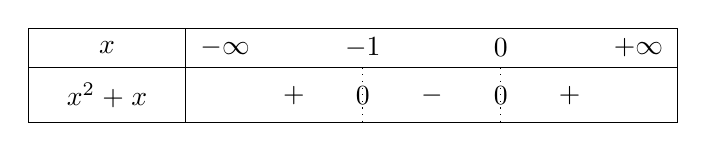
\begin{tikzpicture}[node style/.style={fill opacity=0,text opacity=1}]
        \tkzTabInit[espcl=1.75]{$x$/.5,$x^2 + x$/.7}{$-\infty$,$-1$,$0$,$+\infty$}
        \tkzTabLine{,+,z,-,z,+,}
    \end{tikzpicture}     
\end{itemize}

$$ \text{Donc}\quad
\begin{aligned}
Df & = Df_{1} \cup Df_{2} \\
    & = ]-\infty ; 0] \cup [0 ; +\infty[\\
    &=\mathbb{R} 
\end{aligned}
$$
    
    $$ \textcolor{red}{ \boxed{Df = \mathbb{R}} }$$
  
    \item Déterminons les limites aux bornes de $\mathcal{D}_f$. \hspace{1cm} \textbf{(0,5 pt)}

\begin{itemize}
\item \underline{En $-\infty$}: $f(x)=f_{1}(x)$   
    
\(
\begin{aligned}
 \lim\limits_{x \to -\infty} f(x) &= \lim\limits_{x \to -\infty} \dfrac{x^2-2x}{x-1}\\
 																	&= \lim\limits_{x \to -\infty} \dfrac{x^2}{x}\\
 																	&= \lim\limits_{x \to -\infty} x\\
 																	&= -\infty
\end{aligned}    
\)

\textcolor{red}{{\underline{$\lim\limits_{x \to -\infty} f(x) = -\infty$}}}

\item \underline{En $+\infty$}: $f(x)=f_{2}(x)$   
    
\(
\begin{aligned}
 \lim\limits_{x \to +\infty} f(x) &= \lim\limits_{x \to +\infty} x + \sqrt{x^2+x}\\
 																	&= \lim\limits_{x \to +\infty} x + \sqrt{x^2+x}\\
 																	&= \lim\limits_{x \to +\infty} \\
 																	&= 
\end{aligned}    
\)

\textcolor{red}{{\underline{$\lim\limits_{x \to -\infty} f(x) = -\infty$}}}
\end{itemize}

    \item Étudions la continuité et la dérivabilité de $f$ en $0$. Interprétons les résultats obtenus. \hspace{1cm} \textbf{(1,5 pt)}

 \begin{itemize}
\item \underline{En $0^-$}: $f(x)=f_{1}(x)$   
    
\(
\begin{aligned}
 \lim\limits_{x \to 0^-} f(x) &= \lim\limits_{x \to 0^-} \dfrac{x^2-2x}{x-1}\\
 															&= 0
\end{aligned}    
\)

\textcolor{red}{{\underline{$\lim\limits_{x \to 0^-} f(x) = 0$}}}

\item \underline{En $0^+$}: $f(x)=f_{2}(x)$   
    
\(
\begin{aligned}
 \lim\limits_{x \to 0^+} f(x) &= \lim\limits_{x \to 0^+} x + \sqrt{x^2+x}\\
															&=0
\end{aligned}    
\)

\textcolor{red}{{\underline{$\lim\limits_{x \to 0^+} f(x) = 0$}}}
\end{itemize}   

On a $f(0)=0$

\textcolor{red}{Finalement $\lim\limits_{x \to 0^-} f(x) = \lim\limits_{x \to 0^+} f(x) = f(0)$ donc f est continue en $0$}
    
    \item 
      \begin{enumerate}
        \item Montrons que $(\mathcal{C}_f)$ admet en $-\infty$ une asymptote oblique $\Delta_1$ dont on déterminera l’équation. \textbf{(0,5 pt)}

Comme $\lim\limits_{x \to -\infty} f(x) = -\infty$  

\begin{itemize}
\item Cherchons  $\lim\limits_{x \to -\infty} \dfrac{f(x)}{x} $  

\(
\begin{aligned}
 \lim\limits_{x \to -\infty} \dfrac{f(x)}{x} &= \lim\limits_{x \to -\infty} \dfrac{\dfrac{x^2-2x}{x-1}}{x}\\
 																	&= \lim\limits_{x \to -\infty} \dfrac{x^2-2x}{x^2-x}\\
 																	&= \lim\limits_{x \to -\infty} \dfrac{x^2}{x^2}\\
 																	&= 1
\end{aligned}    
\)        

Donc  $\lim\limits_{x \to -\infty} \dfrac{f(x)}{x} = 1 $       

\item Cherchons  $\lim\limits_{x \to -\infty} f(x)-x $   
\end{itemize}      
        
        \item Étudier la position relative de $(\mathcal{C}_f)$ par rapport à $\Delta_1$ sur $(-\infty;0[$. \hspace{1cm} \textbf{(0,5 pt)}
      \end{enumerate}
    \item Étudier la nature de la branche infinie en $+\infty$. \hspace{1cm} \textbf{(0,5 pt)}
    \item Préciser l'ensemble de dérivabilité de $f$ puis calculer $f'(x)$ sur chaque intervalle où $f$ est dérivable.\\ \textbf{(0,5 pt)}
    \item Dresser le tableau de variation de $f$. \hspace{1cm} \textbf{(0,5 pt)}
    \item Préciser les points d'intersection de $(\mathcal{C}_f)$ avec les axes du repère. \textbf{(0,25 pt)}
    \item Construire la courbe $(\mathcal{C}_f)$. \hspace{1cm} \textbf{(1,5 pt)}
\end{enumerate}

\underline{\textbf{Partie B :}}

Soit $h$ la restriction de $f$ à l’intervalle $I = [0; +\infty[$.

\begin{enumerate}

    \item Montrer que $h$ réalise une bijection de $I$ dans un intervalle $J$ à préciser.
    \hspace{1cm} \textbf{(0,25 pt)}

    \item La bijection réciproque $h^{-1}$ est-elle dérivable sur $J$ ?
    \hspace{1cm} \textbf{(0,25 pt)}

    \item Calculer $h\!\left(\dfrac{4}{5}\right)$ puis $(h^{-1})'(2)$.
   \hspace{1cm} \textbf{(0,5 pt)}

    \item Construire $(\mathcal{C}_{h^{-1}})$ la courbe représentative de $h^{-1}$ dans le même repère.
    \hspace{1cm} \textbf{(0,5 pt)}

    \item Exprimer $h^{-1}(x)$ pour tout $x \in J$.
    \hspace{1cm} \textbf{(0,5 pt)}

\end{enumerate}
+++++++++++++++++++++++++

\underline{\textbf{Partie A :}}

\begin{center}

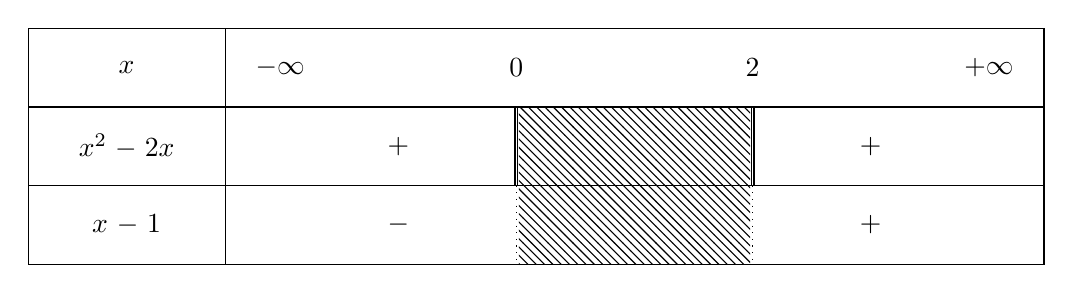
\begin{tikzpicture}
   \tkzTabInit[lgt = 2.5, espcl = 3, deltacl = 0.7]{$x$ / 1 , $x^2-2x$ / 1 , $x-1$ / 1 }{$-\infty$, $0$, $2$, $+\infty$}
   \tkzTabLine{, +, d, h, d, +, }
   \tkzTabLine{, -, t, h, t, +, }
\end{tikzpicture}

\end{center}
\begin{center}
\begin{figure}[H]% Forcer l'image à cet endroit
\centering
\includegraphics[width=0.8\textwidth]{courbe2Devoir1.png}
\caption{Courbe de (Cf)}
\label{fig:monimage}
\end{figure}
\href{https://www.geogebra.org/classic/p6fgutg8}{Clique ici pour voir la courbe sur géogébra}
\end{center}

\end{document}